\documentclass{article}
\usepackage{unicode-math}
\setmainfont{FiraCode-Retina.ttf}
\setmathfont{mathFont.ttf}
\usepackage{tikz}
% \setmathfont[range=\mathit]{fonts/jsMath-cmsy10.ttf}
\begin{document}
Hello $a+b=c$
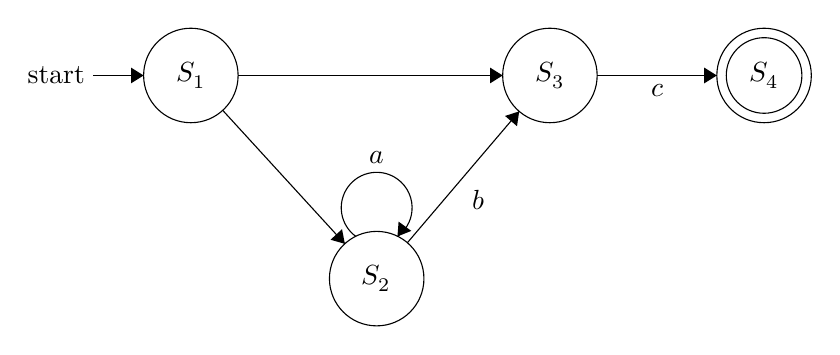
\begin{tikzpicture}[scale=0.2]
        \tikzstyle{every node}+=[inner sep=0pt]
        \draw [black] (25,-24.3) circle (3);
        \draw (25,-24.3) node {$S_1$};
        \draw [black] (36.8,-37.2) circle (3);
        \draw (36.8,-37.2) node {$S_2$};
        \draw [black] (47.8,-24.3) circle (3);
        \draw (47.8,-24.3) node {$S_3$};
        \draw [black] (61.4,-24.3) circle (3);
        \draw (61.4,-24.3) node {$S_4$};
        \draw [black] (61.4,-24.3) circle (2.4);
        \draw [black] (18.8,-24.3) -- (22,-24.3);
        \draw (18.3,-24.3) node [left] {start};
        \fill [black] (22,-24.3) -- (21.2,-23.8) -- (21.2,-24.8);
        \draw [black] (38.75,-34.92) -- (45.85,-26.58);
        \fill [black] (45.85,-26.58) -- (44.95,-26.87) -- (45.71,-27.52);
        \draw (42.85,-32.19) node [right] {$b$};
        \draw [black] (35.477,-34.52) arc (234:-54:2.25);
        \draw (36.8,-29.95) node [above] {$a$};
        \fill [black] (38.12,-34.52) -- (39,-34.17) -- (38.19,-33.58);
        \draw [black] (50.8,-24.3) -- (58.4,-24.3);
        \fill [black] (58.4,-24.3) -- (57.6,-23.8) -- (57.6,-24.8);
        \draw (54.6,-24.8) node [below] {$c$};
        \draw [black] (28,-24.3) -- (44.8,-24.3);
        \fill [black] (44.8,-24.3) -- (44,-23.8) -- (44,-24.8);
        \draw [black] (27.02,-26.51) -- (34.78,-34.99);
        \fill [black] (34.78,-34.99) -- (34.6,-34.06) -- (33.87,-34.73);
      \end{tikzpicture}
\end{document}